\documentclass{extbook}[14pt]
\usepackage{multicol, enumerate, enumitem, hyperref, color, soul, setspace, parskip, fancyhdr, amssymb, amsthm, amsmath, bbm, latexsym, units, mathtools}
\everymath{\displaystyle}
\usepackage[headsep=0.5cm,headheight=0cm, left=1 in,right= 1 in,top= 1 in,bottom= 1 in]{geometry}
\usepackage{dashrule}  % Package to use the command below to create lines between items
\newcommand{\litem}[1]{\item #1

\rule{\textwidth}{0.4pt}}
\pagestyle{fancy}
\lhead{}
\chead{Answer Key for Progress Quiz 3 Version C}
\rhead{}
\lfoot{}
\cfoot{}
\rfoot{Fall 2020}
\begin{document}
\textbf{This key should allow you to understand why you choose the option you did (beyond just getting a question right or wrong). \href{https://xronos.clas.ufl.edu/mac1105spring2020/courseDescriptionAndMisc/Exams/LearningFromResults}{More instructions on how to use this key can be found here}.}

\textbf{If you have a suggestion to make the keys better, \href{https://forms.gle/CZkbZmPbC9XALEE88}{please fill out the short survey here}.}

\textit{Note: This key is auto-generated and may contain issues and/or errors. The keys are reviewed after each exam to ensure grading is done accurately. If there are issues (like duplicate options), they are noted in the offline gradebook. The keys are a work-in-progress to give students as many resources to improve as possible.}

\rule{\textwidth}{0.4pt}

\begin{enumerate}\litem{
Describe the end behavior of the polynomial below.
\[ f(x) = -8(x + 9)^{4}(x - 9)^{5}(x - 2)^{5}(x + 2)^{6} \]
The solution is the graph below, which is option B.
\begin{center}
    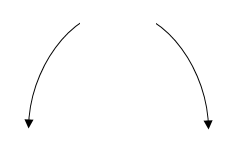
\includegraphics[width=0.3\textwidth]{../Figures/polyEndBehaviorBC.png}
\end{center}\begin{enumerate}[label=\Alph*.]
\begin{multicols}{2}
\item 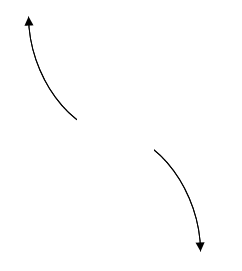
\includegraphics[width = 0.3\textwidth]{../Figures/polyEndBehaviorAC.png}
\item 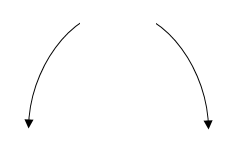
\includegraphics[width = 0.3\textwidth]{../Figures/polyEndBehaviorBC.png}
\item 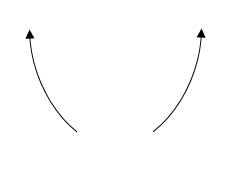
\includegraphics[width = 0.3\textwidth]{../Figures/polyEndBehaviorCC.png}
\item 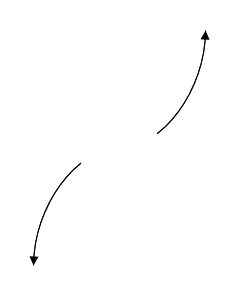
\includegraphics[width = 0.3\textwidth]{../Figures/polyEndBehaviorDC.png}
\end{multicols}\item None of the above.\end{enumerate}
\textbf{General Comment:} Remember that end behavior is determined by the leading coefficient AND whether the \textbf{sum} of the multiplicities is positive or negative.
}
\litem{
Describe the zero behavior of the zero $x = 2$ of the polynomial below.
\[ f(x) = -5(x + 8)^{9}(x - 8)^{5}(x - 2)^{6}(x + 2)^{5} \]
The solution is the graph below, which is option C.
\begin{center}
    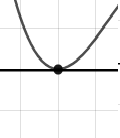
\includegraphics[width=0.3\textwidth]{../Figures/polyZeroBehaviorCC.png}
\end{center}\begin{enumerate}[label=\Alph*.]
\begin{multicols}{2}
\item 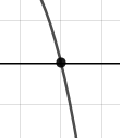
\includegraphics[width = 0.3\textwidth]{../Figures/polyZeroBehaviorAC.png}
\item 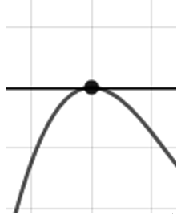
\includegraphics[width = 0.3\textwidth]{../Figures/polyZeroBehaviorBC.png}
\item 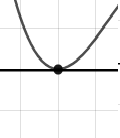
\includegraphics[width = 0.3\textwidth]{../Figures/polyZeroBehaviorCC.png}
\item 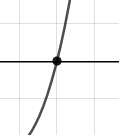
\includegraphics[width = 0.3\textwidth]{../Figures/polyZeroBehaviorDC.png}
\end{multicols}\item None of the above.\end{enumerate}
\textbf{General Comment:} You will need to sketch the entire graph, then zoom in on the zero the question asks about.
}
\litem{
Which of the following equations \textit{could} be of the graph presented below?

\begin{center}
    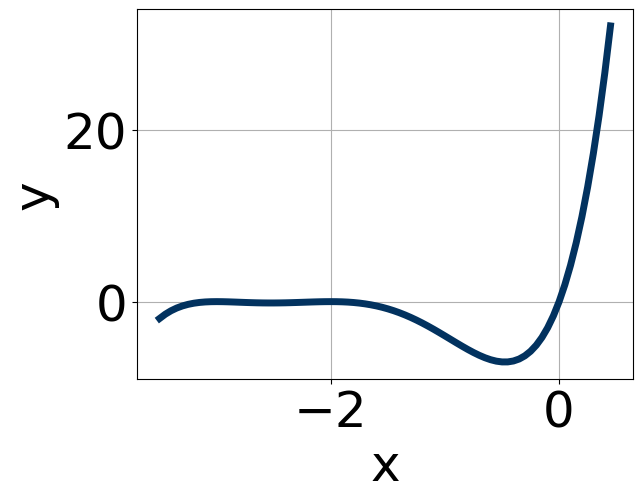
\includegraphics[width=0.5\textwidth]{../Figures/polyGraphToFunctionCopyC.png}
\end{center}



The solution is \( 12x^{7} (x + 3)^{10} (x + 2)^{4} \), which is option A.\begin{enumerate}[label=\Alph*.]
\item \( 12x^{7} (x + 3)^{10} (x + 2)^{4} \)

* This is the correct option.
\item \( 14x^{8} (x + 3)^{6} (x + 2)^{5} \)

The factor $(x + 2)$ should have an even power and the factor $x$ should have an odd power.
\item \( -5x^{6} (x + 3)^{4} (x + 2)^{6} \)

The factor $x$ should have an odd power and the leading coefficient should be the opposite sign.
\item \( 15x^{5} (x + 3)^{6} (x + 2)^{7} \)

The factor $(x + 2)$ should have an even power.
\item \( -17x^{5} (x + 3)^{6} (x + 2)^{6} \)

This corresponds to the leading coefficient being the opposite value than it should be.
\end{enumerate}

\textbf{General Comment:} General Comments: Draw the x-axis to determine which zeros are touching (and so have even multiplicity) or cross (and have odd multiplicity).
}
\litem{
Describe the end behavior of the polynomial below.
\[ f(x) = -3(x - 5)^{4}(x + 5)^{5}(x + 9)^{3}(x - 9)^{4} \]
The solution is the graph below, which is option B.
\begin{center}
    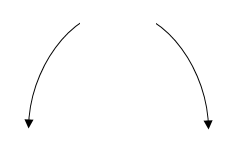
\includegraphics[width=0.3\textwidth]{../Figures/polyEndBehaviorCopyBC.png}
\end{center}\begin{enumerate}[label=\Alph*.]
\begin{multicols}{2}
\item 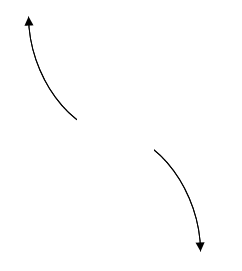
\includegraphics[width = 0.3\textwidth]{../Figures/polyEndBehaviorCopyAC.png}
\item 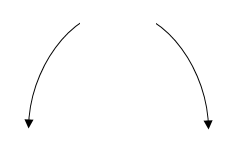
\includegraphics[width = 0.3\textwidth]{../Figures/polyEndBehaviorCopyBC.png}
\item 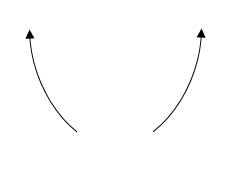
\includegraphics[width = 0.3\textwidth]{../Figures/polyEndBehaviorCopyCC.png}
\item 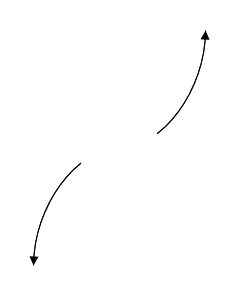
\includegraphics[width = 0.3\textwidth]{../Figures/polyEndBehaviorCopyDC.png}
\end{multicols}\item None of the above.\end{enumerate}
\textbf{General Comment:} Remember that end behavior is determined by the leading coefficient AND whether the \textbf{sum} of the multiplicities is positive or negative.
}
\litem{
Construct the lowest-degree polynomial given the zeros below. Then, choose the intervals that contain the coefficients of the polynomial in the form $x^3+bx^2+cx+d$.
\[ -5 + 2 i \text{ and } -2 \]
The solution is \( x^{3} +12 x^{2} +49 x + 58 \), which is option B.\begin{enumerate}[label=\Alph*.]
\item \( b \in [0, 3], c \in [-4, 3], \text{ and } d \in [-7, -1] \)

$x^{3} + x^{2} -4$, which corresponds to multiplying out $(x -2)(x + 2)$.
\item \( b \in [11, 17], c \in [48, 50], \text{ and } d \in [57, 61] \)

* $x^{3} +12 x^{2} +49 x + 58$, which is the correct option.
\item \( b \in [0, 3], c \in [4, 10], \text{ and } d \in [3, 13] \)

$x^{3} + x^{2} +7 x + 10$, which corresponds to multiplying out $(x + 5)(x + 2)$.
\item \( b \in [-13, -10], c \in [48, 50], \text{ and } d \in [-61, -53] \)

$x^{3} -12 x^{2} +49 x -58$, which corresponds to multiplying out $(x-(-5 + 2 i))(x-(-5 - 2 i))(x -2)$.
\item \( \text{None of the above.} \)

This corresponds to making an unanticipated error or not understanding how to use nonreal complex numbers to create the lowest-degree polynomial. If you chose this and are not sure what you did wrong, please contact the coordinator for help.
\end{enumerate}

\textbf{General Comment:} Remember that the conjugate of $a+bi$ is $a-bi$. Since these zeros always come in pairs, we need to multiply out $(x-(-5 + 2 i))(x-(-5 - 2 i))(x-(-2))$.
}
\litem{
Construct the lowest-degree polynomial given the zeros below. Then, choose the intervals that contain the coefficients of the polynomial in the form $ax^3+bx^2+cx+d$.
\[ \frac{1}{3}, \frac{2}{5}, \text{ and } \frac{1}{2} \]
The solution is \( 30x^{3} -37 x^{2} +15 x -2 \), which is option E.\begin{enumerate}[label=\Alph*.]
\item \( a \in [29, 32], b \in [36, 40], c \in [10, 16], \text{ and } d \in [0.7, 3.2] \)

$30x^{3} +37 x^{2} +15 x + 2$, which corresponds to multiplying out $(3x + 1)(5x + 2)(2x + 1)$.
\item \( a \in [29, 32], b \in [1, 12], c \in [-11, -6], \text{ and } d \in [-2.2, -0.1] \)

$30x^{3} +7 x^{2} -7 x -2$, which corresponds to multiplying out $(3x + 3)(5x + 5)(2x -2)$.
\item \( a \in [29, 32], b \in [-40, -33], c \in [10, 16], \text{ and } d \in [0.7, 3.2] \)

$30x^{3} -37 x^{2} +15 x + 2$, which corresponds to multiplying everything correctly except the constant term.
\item \( a \in [29, 32], b \in [-21, -15], c \in [-3, 0], \text{ and } d \in [0.7, 3.2] \)

$30x^{3} -17 x^{2} -3 x + 2$, which corresponds to multiplying out $(3x + 3)(5x -5)(2x -2)$.
\item \( a \in [29, 32], b \in [-40, -33], c \in [10, 16], \text{ and } d \in [-2.2, -0.1] \)

* $30x^{3} -37 x^{2} +15 x -2$, which is the correct option.
\end{enumerate}

\textbf{General Comment:} To construct the lowest-degree polynomial, you want to multiply out $(3x -1)(5x -2)(2x -1)$
}
\litem{
Construct the lowest-degree polynomial given the zeros below. Then, choose the intervals that contain the coefficients of the polynomial in the form $ax^3+bx^2+cx+d$.
\[ \frac{2}{5}, \frac{-7}{5}, \text{ and } 3 \]
The solution is \( 25x^{3} -50 x^{2} -89 x + 42 \), which is option A.\begin{enumerate}[label=\Alph*.]
\item \( a \in [22, 30], b \in [-53, -44], c \in [-89, -85], \text{ and } d \in [32, 48] \)

* $25x^{3} -50 x^{2} -89 x + 42$, which is the correct option.
\item \( a \in [22, 30], b \in [-53, -44], c \in [-89, -85], \text{ and } d \in [-44, -39] \)

$25x^{3} -50 x^{2} -89 x -42$, which corresponds to multiplying everything correctly except the constant term.
\item \( a \in [22, 30], b \in [-30, -29], c \in [-128, -119], \text{ and } d \in [-44, -39] \)

$25x^{3} -30 x^{2} -121 x -42$, which corresponds to multiplying out $(5x + 5)(5x -5)(x -1)$.
\item \( a \in [22, 30], b \in [50, 51], c \in [-89, -85], \text{ and } d \in [-44, -39] \)

$25x^{3} +50 x^{2} -89 x -42$, which corresponds to multiplying out $(5x + 2)(5x -7)(x + 3)$.
\item \( a \in [22, 30], b \in [-108, -96], c \in [60, 64], \text{ and } d \in [32, 48] \)

$25x^{3} -100 x^{2} +61 x + 42$, which corresponds to multiplying out $(5x + 5)(5x + 5)(x -1)$.
\end{enumerate}

\textbf{General Comment:} To construct the lowest-degree polynomial, you want to multiply out $(5x -2)(5x + 7)(x -3)$
}
\litem{
Construct the lowest-degree polynomial given the zeros below. Then, choose the intervals that contain the coefficients of the polynomial in the form $x^3+bx^2+cx+d$.
\[ -3 + 2 i \text{ and } -3 \]
The solution is \( x^{3} +9 x^{2} +31 x + 39 \), which is option C.\begin{enumerate}[label=\Alph*.]
\item \( b \in [-2, 6], c \in [2, 11], \text{ and } d \in [7, 14] \)

$x^{3} + x^{2} +6 x + 9$, which corresponds to multiplying out $(x + 3)(x + 3)$.
\item \( b \in [-2, 6], c \in [1, 2], \text{ and } d \in [-12, 2] \)

$x^{3} + x^{2} +x -6$, which corresponds to multiplying out $(x -2)(x + 3)$.
\item \( b \in [5, 21], c \in [23, 38], \text{ and } d \in [39, 45] \)

* $x^{3} +9 x^{2} +31 x + 39$, which is the correct option.
\item \( b \in [-10, -8], c \in [23, 38], \text{ and } d \in [-40, -33] \)

$x^{3} -9 x^{2} +31 x -39$, which corresponds to multiplying out $(x-(-3 + 2 i))(x-(-3 - 2 i))(x -3)$.
\item \( \text{None of the above.} \)

This corresponds to making an unanticipated error or not understanding how to use nonreal complex numbers to create the lowest-degree polynomial. If you chose this and are not sure what you did wrong, please contact the coordinator for help.
\end{enumerate}

\textbf{General Comment:} Remember that the conjugate of $a+bi$ is $a-bi$. Since these zeros always come in pairs, we need to multiply out $(x-(-3 + 2 i))(x-(-3 - 2 i))(x-(-3))$.
}
\litem{
Describe the zero behavior of the zero $x = 8$ of the polynomial below.
\[ f(x) = 2(x + 3)^{13}(x - 3)^{9}(x + 8)^{12}(x - 8)^{7} \]
The solution is the graph below, which is option D.
\begin{center}
    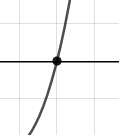
\includegraphics[width=0.3\textwidth]{../Figures/polyZeroBehaviorCopyDC.png}
\end{center}\begin{enumerate}[label=\Alph*.]
\begin{multicols}{2}
\item 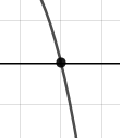
\includegraphics[width = 0.3\textwidth]{../Figures/polyZeroBehaviorCopyAC.png}
\item 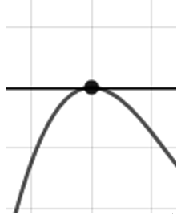
\includegraphics[width = 0.3\textwidth]{../Figures/polyZeroBehaviorCopyBC.png}
\item 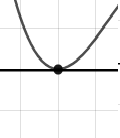
\includegraphics[width = 0.3\textwidth]{../Figures/polyZeroBehaviorCopyCC.png}
\item 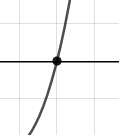
\includegraphics[width = 0.3\textwidth]{../Figures/polyZeroBehaviorCopyDC.png}
\end{multicols}\item None of the above.\end{enumerate}
\textbf{General Comment:} You will need to sketch the entire graph, then zoom in on the zero the question asks about.
}
\litem{
Which of the following equations \textit{could} be of the graph presented below?

\begin{center}
    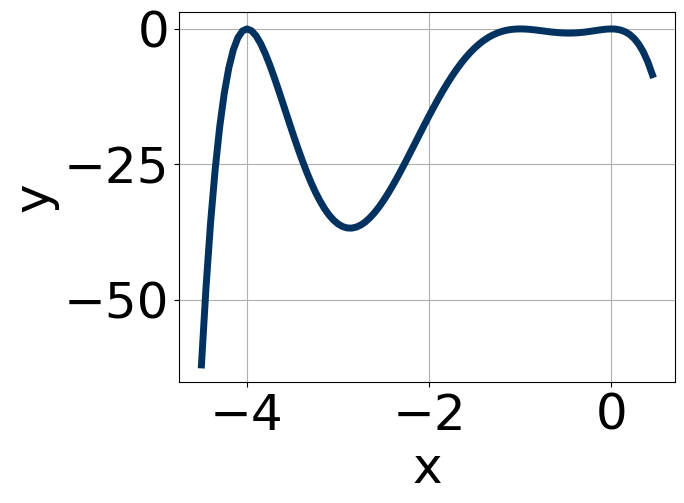
\includegraphics[width=0.5\textwidth]{../Figures/polyGraphToFunctionC.png}
\end{center}



The solution is \( -19x^{4} (x + 4)^{6} (x + 1)^{4} \), which is option B.\begin{enumerate}[label=\Alph*.]
\item \( 19x^{10} (x + 4)^{4} (x + 1)^{5} \)

The factor $(x + 1)$ should have an even power and the leading coefficient should be the opposite sign.
\item \( -19x^{4} (x + 4)^{6} (x + 1)^{4} \)

* This is the correct option.
\item \( -18x^{8} (x + 4)^{10} (x + 1)^{11} \)

The factor $(x + 1)$ should have an even power.
\item \( -11x^{7} (x + 4)^{6} (x + 1)^{5} \)

The factors $x$ and $(x + 1)$ should both have even powers.
\item \( 4x^{4} (x + 4)^{8} (x + 1)^{10} \)

This corresponds to the leading coefficient being the opposite value than it should be.
\end{enumerate}

\textbf{General Comment:} General Comments: Draw the x-axis to determine which zeros are touching (and so have even multiplicity) or cross (and have odd multiplicity).
}
\end{enumerate}

\end{document}